\documentclass[10pt,a4paper]{article}
\usepackage[latin1]{inputenc}
\usepackage{amsmath}
\usepackage{amsfonts}
\usepackage{amssymb}
\usepackage{fullpage}
\usepackage{graphicx}
\usepackage{parskip}

\begin{document}
\title{J.D. Jackson Problem 1.7}
\author{Josh Orndorff \\ admin@joshorndorff.com}
\maketitle

\section{Capacitance per unit Length}
Let's note right away that Jackson is using the symbol $C$ to represent capacitance per unit length. This is contrary to the standard that $C$ is capacitance. I will follow the standard and solve for $C/L$ as capacitance per unit length.
\begin{figure}[h]
\centering
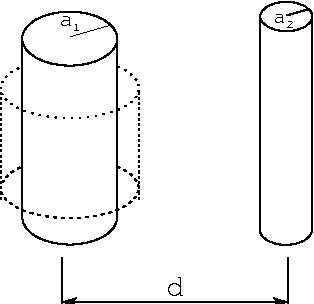
\includegraphics[scale=.9]{Jackson1-7.png}
\caption{The geometry of the problem. Both cylinders are infinitely long. The dotted surface is a finite cylindrical Gaussian surface. Let the left cylinder be centered on $x=0$ with charge density $+\lambda$ and the right on $x=d$ with $-\lambda$.}
\end{figure}

In order to find the electric field due to the left cylinder, we can use Gauss's law for the dashed surface indicated. We know by symmetry that it is directed radially outward.
\begin{equation}
\oint_S \mathbf{E_1}\cdot d\mathbf{A} = \frac{q_{enc}}{\epsilon_0}
\end{equation}
\begin{equation}
2\pi r l E_1= \frac{\lambda l}{\epsilon_0}
\end{equation}
\begin{equation}
\mathbf{E_1}= \frac{\lambda}{2\pi r \epsilon_0}\hat{r}
\end{equation}

There was nothing special about the left cylinder, and by the same method we can see that the field due to the right cylinder is
\begin{equation}
\mathbf{E_2}= \frac{-\lambda}{2\pi r_2 \epsilon_0}\hat{r}_2
\end{equation}
(I'm using the subscript two here to indicate a coordinate system that is actually centered on the second cylinder.)

I've intentionally avoided being totally rigorous (and all the notation that comes along with such rigor) expressing the fields because the region that we care about is just a line between the cylinders.  Along this line, we only need to worry about one coordinate, $x$, and we can note that the two fields are exactly parallel and facing to the right.
\begin{equation}
E=E_1+E_2=\frac{\lambda}{2\pi x \epsilon_0}+\frac{\lambda}{2\pi (d-x) \epsilon_0}
\end{equation}

\begin{equation}
E=\frac{\lambda}{2\pi\epsilon_0}\left[\frac{1}{x}+\frac{1}{d-x}\right]
\end{equation}

Next we need to find the electric potential difference between the two conductors, so we'll do a line integral along the straight line between them.
\begin{equation}
V=\int_{a_1}^{d-a_2}\frac{\lambda}{2\pi\epsilon_0}\left[\frac{1}{x}+\frac{1}{d-x}\right]\,\mathrm{d}x
\end{equation}
\begin{equation}
V=\frac{\lambda}{2\pi\epsilon_0}\left[\ln x - \ln d-x \right]_{a_1}^{d-a_2}
\end{equation}
\begin{equation}
V=\frac{\lambda}{2\pi\epsilon_0}\left[\ln \frac{x}{d-x} \right]_{a_1}^{d-a_2}
\end{equation}
\begin{equation}
V=\frac{\lambda}{2\pi\epsilon_0}\left[\ln \frac{a_1}{d-a_1} - \ln \frac{d-a_2}{d-(d-a_2)} \right]
\end{equation}
\begin{equation}
V=\frac{\lambda}{2\pi\epsilon_0}\ln \frac{a_1 a_2}{(d-a_1)(d-a_2)}
\end{equation}

Jackson defines for us the geometric mean $a^2=a_1a_2$ which we can substitute into the numerator. He also tells us that $d \gg a_1$, $d \gg a_2$ which means we can replace each binomial in the denominator with just $d$.
\begin{equation}
V \approx \frac{\lambda}{2\pi\epsilon_0}\ln \frac{a^2}{d^2}
\end{equation}

Next, using logarithm properties, 
\begin{equation}
V \approx \frac{\lambda}{\pi\epsilon_0}\ln \frac{a}{d}
\end{equation}

Finally we can use our charge density and the newly-found expression for potential difference in to find capacitance. $C/L=\lambda/V$
\begin{equation}
\frac{C}{L}\approx \frac{\pi\epsilon_0}{\ln(d/a)}
\end{equation}

If you're concerned about my flipping the ratio in the natural log, remember that capacitance is a positive definite quantity, and $\ln(a/d)=-\ln(d/a)$.

Finally the values that Jackson requested.
\begin{table}[h]\centering
    \begin{tabular}{|l|l|l|}
        \hline
        d (separation) & a (radius) & 2a (diameter) \\ \hline
        .5 cm          & .492 mm    & .985 mm       \\ 
        1.5 cm         & 1.477 cm   & 2.95 mm       \\ 
        5 cm           & 4.923 cm   & 9.85 mm       \\
        \hline
    \end{tabular}
\end{table}
\end{document}